\documentclass{article}

\usepackage{neurips_2026}

\usepackage[utf8]{inputenc}
\usepackage[T1]{fontenc}
\usepackage{hyperref}
\usepackage{url}
\usepackage{booktabs}
\usepackage{amsfonts}
\usepackage{amssymb}
\usepackage{amsmath}
\usepackage{nicefrac}
\usepackage{microtype}
\usepackage{xcolor}
\usepackage{graphicx}
\usepackage{array}
\usepackage{enumitem}
\usepackage{placeins}

\newcommand{\method}[1]{\texttt{#1}}
\newcommand{\wstar}{W^{\star}}
\newcommand{\rwstar}{RW^{\star}}
\newcommand{\mstar}{M^{\star}}
\newcommand{\cstar}{C^{\star}}
\newcommand{\phiroute}{\varphi_{\mathrm{route}}}

% TODO(camera-ready): venue retarget; cite the three companion papers
% (Q/R/M/C framework, collective semantic memory, semantic warp) per the
% venue's concurrent-submission policy.

\title{The Song, Not the Pin: Route Transfer and\\Meaning-Based Place Identity in Collective Memory}

%\author{%
%  Anonymous Authors \\
%}

\begin{document}

\maketitle

\begin{abstract}
\textbf{Problem.} The companion warp paper measures whether an agent can reach a target known only from a peer's memory. Two assumptions remain hidden in that construction --- and in essentially all shared-memory multi-agent systems. First, what transfers is a \emph{point}: broadcast snapshots carry place summaries but no edges, so the traveler learns WHERE and must re-derive HOW. Second, place identity is a \emph{shared coordinate frame}: `the same place' means `close $(x,y)$ in a grid the environment hands to every agent'; semantics only breaks ties inside a spatial radius. In the source culture a songline is neither: the song IS the route, and its places are identified by what they look like, not by coordinates nobody shares.
\textbf{Approach.} We remove both assumptions and measure what each was hiding. (i) \emph{Route warp}: broadcasts carry traversed edges with provenance; $\phiroute$ is the foreign share of edge mass along the committed path, and a strict $\rwstar$ is a connected foreign sub-path the traveler has never walked. (ii) \emph{Semantic place identity}: places are matched by local semantic constellations (translation-invariant fingerprints); the inter-agent frame --- translation in one step, full $SE(2)$ with rotations in the next --- is recovered from mutually-unique matches of co-visited landmarks, and foreign evidence, including never-seen targets, is transported through it.
\textbf{Findings.} What route knowledge buys is a step function, not a slope: place-only transfer collapses at the FIRST wall (success $1.0$ at detour $D{=}1.00$ vs.\ $0.0$ at $D{=}1.38$, and worse than blind exploration), while route transfer completes everywhere. Aging breaks the transferred route at a point predictable to the exact edge ($110/110$ regimes; all $40$ mid-route ruptures across two world classes at the predicted index, error $0$), and safety travels with the route: $0$ hazard hits over the witness's path vs.\ $3.25$ $[2.45,4.10]$ for the place-only traveler, with the risk RESUMING at the predicted rupture point. Meaning-based identity recovers secret frames exactly ($100\%$ translation; $80/80$ under $SE(2)$), restores $88\%$ of the shared-frame performance in the full peer stack, and fails \emph{closed} under perceptual aliasing where the coordinate assumption fails \emph{open} --- and the companion distance law re-emerges tick-exactly (breakpoints $20/14/9$) with no shared origin and no shared north.
\textbf{Thesis.} A shared map is not what makes collective navigation work. What transfers is the song --- a sequence with meaning-anchored places --- and each impoverishment of the song (point instead of route, coordinates instead of meaning) fails in a specific, measurable, and now predicted way.
\textbf{Scope.} Grid worlds; translation and $90^\circ$ rotations; measurement and minimal mechanisms, not a general theory.
\end{abstract}

\section{Introduction}
\label{sec:intro}

A songline encodes a journey: a sequence of places, each recognisable
by what is there, bound into a path by the song's order. When
multi-agent systems ``share memory,'' they typically share something
much poorer --- a pin on a common map: coordinates of a target in a
frame all agents are assumed to inhabit. The companion warp
paper\footnote{Companion submissions: the Q/R/M/C measurement
framework, the collective-semantic-memory architecture study, and the
semantic-warp measurement paper. Citations deferred per
concurrent-submission policy.} made the act of navigating by someone
else's memory a measured event ($\wstar$: a materialisation whose
evidence is entirely foreign) and showed its value is governed by the
coordination contract attached to the information. But its
construction inherited the two impoverishments silently:

\begin{enumerate}[leftmargin=20pt,itemsep=2pt,topsep=2pt]
\item \textbf{The pin, not the song.} Broadcast snapshots carry place
  concepts --- centroids, tags, confidences --- but no edges. The
  receiver learns WHERE the water is; the route is re-derived from
  scratch. In open grids this is invisible: the manhattan path is the
  route. The moment paths are expensive, it is everything.
\item \textbf{Coordinates, not meaning.} `Same place' is operationalised
  as coordinate proximity, with semantics as a tie-breaker inside a
  radius. The cross-agent place-correspondence problem --- the reason
  map merging is hard in robotics --- is bracketed by fiat.
\end{enumerate}

This paper removes both assumptions, one at a time, with the
measurement discipline of the series: every claim is registered before
the runs, failures against registration are reported with their
mechanisms, and the strongest results are exact-match validations of
closed-form predictions.

\paragraph{Contributions.}
\begin{enumerate}[leftmargin=20pt,itemsep=2pt,topsep=2pt]
\item \textbf{Route warp} ($\rwstar$, $\phiroute$): edge-level
  provenance and the strict route-warp event --- a connected foreign
  sub-path the traveler never walked (\S\ref{sec:route}). The value of
  route over place transfer is a \emph{cliff}, not a slope: place-only
  transfer dies at the first wall ($1.0 \to 0.0$ success between
  measured detour $1.00$ and $1.38$) and is WORSE than no transfer at
  all there, while route transfer completes everywhere
  (\S\ref{sec:cliff}).
\item \textbf{The rupture law}: a witness stamps edges sequentially,
  so its trace ages non-uniformly and a delayed traveler chases a
  fading song. Replaying the series' trust$\times$staleness gate over
  calibrated kinematics predicts \emph{where the song breaks} to the
  exact edge: $110/110$ regime matches, all $21$ mid-route ruptures at
  the predicted index (error $0$), and a discrete trust-flip that
  zeroes route commits entirely (\S\ref{sec:rupture}).
\item \textbf{Hazard stratification}: the wall and hazard axes are
  independent --- walls break place-transfer's \emph{completion},
  hazards break its \emph{safety} ($0$ vs.\ $3.25$ hits at equal
  completion and $+0.7$ ticks), and when the song ruptures the risk
  resumes at the predicted edge (\S\ref{sec:hazard}).
\item \textbf{Meaning-based place identity}: translation-invariant
  semantic fingerprints, mutually-unique landmark matching, and
  consensus frame recovery --- translation first, full $SE(2)$ with
  secret $90^\circ$ rotations after (\S\ref{sec:identity}). Exact
  frame recovery ($100\%$; $80/80$ under $SE(2)$); online alignment in
  the full peer stack recovering $88\%$ of the shared-frame gap; a
  proved failure asymmetry (semantic identity fails \emph{closed}
  under aliasing and under in-principle-unrecoverable $180^\circ$
  symmetry; coordinate identity fails \emph{open}); and the companion
  distance law reproduced tick-exactly ($20/14/9$) with no shared
  frame at all (\S\ref{sec:stack}).
\end{enumerate}

\section{Setting}
\label{sec:setting}

Grid worlds ($12{\times}10$ to $14{\times}12$) with semantic water
targets, hazards, and walls; agents with symbolic place memory,
peer broadcast on cadence $K$, and the series' standard planner
(target lock $=$ the Q/R/M/C $\mstar$ event; completion $\cstar$).
The trust$\times$staleness inclusion rule of the collective-memory
companion is used throughout with unchanged constants: evidence
mass $\text{trust}\cdot e^{-\alpha\,\text{age}}\cdot m$, threshold
$\tau{=}0.30$, $\alpha{=}0.05$. Warp events follow the companion warp
paper: provenance $\varphi$ frozen at lock time; completion attributed
to a continuous lock from a foreign commit ($\varphi{=}1$ at first
lock) to success. % TODO: compress; cross-reference companions.

\section{Route warp: transferring the HOW}
\label{sec:route}

\paragraph{Edge provenance.} Broadcast snapshots additionally carry the
sender's OWN traversed edges $(a,b,\text{count},\text{last tick})$;
foreign edges are never re-broadcast (the same privacy contract as
place snapshots: no agent reads another's graph, transport only). For
the path $P$ a planner commits,
\[
\phiroute(P) \;=\;
\frac{\sum_{e\in P,\;\pi(e)\neq\mathrm{self}} w(e)}
     {\sum_{e\in P} w(e)},
\qquad w(e) = \text{trust}\cdot e^{-\alpha\,\text{age}(e)}\cdot
\log(1{+}\text{count}(e)),
\]
the same weights the route gate uses. A \textbf{strict $\rwstar$} is a
committed, traversed, connected sub-path of $\ge 5$ edges with
$\phiroute = 1$: the whole verse is someone else's. Place warp is the
degenerate case (path length $0$: only the target is foreign), giving
a two-dimensional provenance plane $(\varphi_{\mathrm{place}},
\phiroute)$.

\paragraph{First strict $\rwstar$.} On a comb maze with measured
detour $D{=}2.65$, a traveler commits and walks a fully foreign
$45$-edge route to completion in $54$ ticks; with the same foreign
PLACE evidence but no edges, the standard planner never arrives
(300-tick budget), and blind exploration takes $126$.

\subsection{The cliff: what route knowledge buys}
\label{sec:cliff}

\begin{figure}[t]
\centering
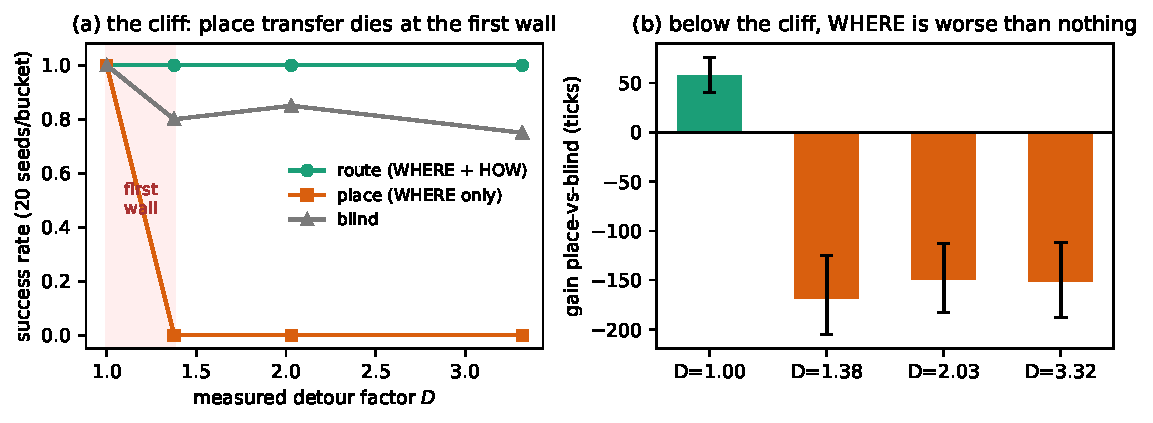
\includegraphics[width=\linewidth]{figures/fig_route_cliff}
\caption{The cliff (paired arms on identical mazes, 20 seeds per
measured-detour bucket). \textbf{(a)} Place-only transfer does not
degrade with detour --- it collapses at the FIRST wall, located by the
probe bucket between $D{=}1.00$ and $D{=}1.38$; route transfer
completes everywhere. \textbf{(b)} Below the cliff, knowing WHERE
without HOW is \emph{worse than knowing nothing}: the known-target
manhattan pull pins the planner against walls ($-150$ to $-168$ ticks
vs.\ blind exploration), while in the open world the same knowledge is
worth $+57$.}
\label{fig:cliff}
\end{figure}

\begin{table}[h]
\centering
\caption{Three arms on identical mazes (paired by seed), bucketed by
MEASURED detour factor $D$; 20 seeds per bucket, censored gains
(fail $=300$). Place-only transfer does not degrade with $D$ --- it
collapses at the first wall, and is worse than blind exploration
there (the known-target manhattan pull pins the planner against
walls). Route transfer completes everywhere; every completion is a
strict $\rwstar$ with $\phiroute=1$.}
\label{tab:cliff}
\small
\begin{tabular}{lcccc}
\toprule
$D$ & gain route-vs-place [CI] & gain route-vs-blind [CI] & succ r/p/b \\
\midrule
1.00 & $+4.7$ $[+3.4,+6.0]$ & $+62$ $[+44,+80]$ & 20/\textbf{20}/20 \\
1.38 & $+281$ $[+279,+283]$ & $+113$ $[+77,+155]$ & 20/\textbf{0}/16 \\
2.03 & $+273$ $[+271,+275]$ & $+123$ $[+91,+160]$ & 20/\textbf{0}/17 \\
3.32 & $+262$ $[+259,+264]$ & $+110$ $[+72,+152]$ & 20/\textbf{0}/15 \\
\bottomrule
\end{tabular}
\end{table}

Figure~\ref{fig:cliff} shows both faces of the result.
Two pre-registered predictions failed here, in instructive ways.
The negative control at $D{=}1$ was registered in ticks
($|\text{gain}|\le 3$) and came out $+4.7$: the gap is \emph{turn
economy} (BFS routes walk straight legs; the dominant-axis planner
alternates axes), not route knowledge --- in path LENGTH the gap is
exactly $0.0$ $[0.0,0.0]$ across all 20 open-grid cells. And ``gain
grows with $D$'' is unmeasurable: with place success at $0$ the gain
saturates at the censoring ceiling. The correct form of the law is a
step located by the probe bucket at $D\in(1.00,1.38)$, i.e.\ the
first wall. % re-registration documented in the artifact.

\section{The rupture law: where the song breaks}
\label{sec:rupture}

The witness stamps edge $i$ at tick $i$: its trace ages
non-uniformly, the start of the route always older than the end, and
a traveler delayed by $a_0$ \emph{chases a fading song}. Under the
standard gate the binding edge is the CURRENT one (the oldest
remaining), giving three regimes on the $a_0$ axis: complete;
rupture at a predictable path index; dead on arrival. The predictor
is fully deterministic --- a no-decay calibration run records the
traveler's kinematics (path index per tick, turns included), and the
registered prediction replays the closed-form gate over that
trajectory, the same device that produced the companion paper's
$6/6$ hold-out.

Across 5 mazes $\times$ 11 delays $\times$ 2 trusts (110 cells,
registered before execution): \textbf{110/110 regime matches; all 21
mid-route ruptures at exactly the predicted edge index (error $0$)};
and a route trust-flip --- at trust $0.7$ the single-traversal edge
mass gives $\mathrm{age}_{\max} = 9.6 < L$, so \emph{no route ever
commits} (0 commits observed; the discrete off-switch of the
companion law, now for paths). The rupture of a transferred route is
thus not noise but a law: the same constants
$(\alpha,\tau,\text{trust})$ that set WHEN a place-warp gate closes
set WHERE a route-warp breaks.

\section{Hazard stratification: the song protects}
\label{sec:hazard}

\begin{table}[h]
\centering
\caption{Open fields dense with passable-but-punished hazards
(density $0.20$), the witness's route hazard-avoiding by experience;
20 paired worlds, decay off (the safety axis isolated from the aging
axis). Both transfer modes COMPLETE --- the wall axis
(Table~\ref{tab:cliff}) and the hazard axis are independent; they
differ in the price.}
\label{tab:hazard}
\small
\begin{tabular}{lccc}
\toprule
Arm & hazard hits [CI] & completion & mean $t$ \\
\midrule
route (foreign safe path) & \textbf{0} (all 20 cells) & 20/20 & 16.6 \\
place (WHERE only) & 3.25 $[2.45, 4.10]$ & 20/20 & 15.9 \\
blind & 28.7 & --- & --- \\
\bottomrule
\end{tabular}
\end{table}

\begin{figure}[t]
\centering
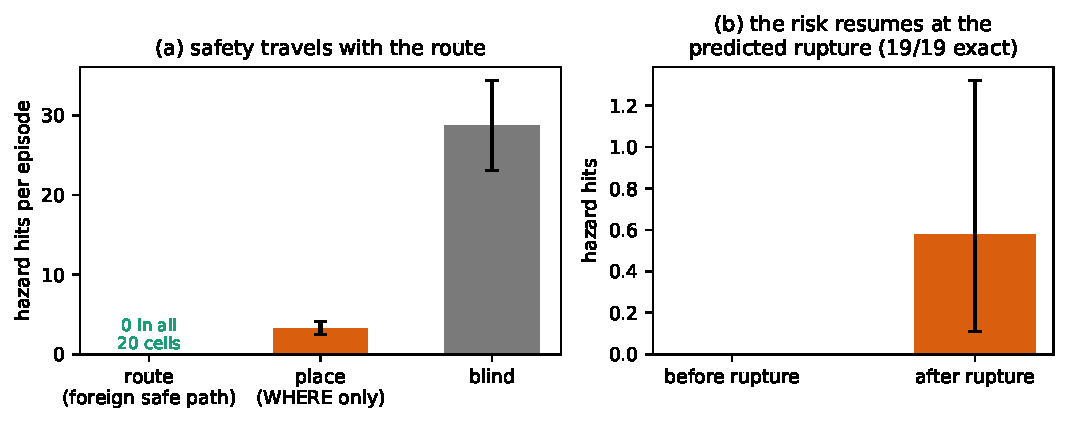
\includegraphics[width=0.92\linewidth]{figures/fig_route_hazard}
\caption{The song protects. \textbf{(a)} Hazard hits per episode: the
traveler on the witness's route inherits its safety outright ($0$ in
all 20 worlds); the place-only traveler pays $3.25$ hits for the same
completion; blind exploration pays $28.7$. \textbf{(b)} Composition
with the rupture law: in the rupture regime the traveler takes zero
hits while the song lasts, and the risk resumes after the break ---
which occurs at the R2-predicted edge index in all $19/19$ cells.}
\label{fig:hazard}
\end{figure}

The traveler following the witness's path inherits its safety
outright, at a time premium of $+0.7$ ticks
(Figure~\ref{fig:hazard}a). Composing with \S\ref{sec:rupture}: in the rupture regime (19/20 worlds) the
traveler takes \textbf{0 hits before the rupture} and $0.58$
$[0.11,1.32]$ after it, when it falls back on place knowledge and
re-enters the field --- with all 19 ruptures again at the
R2-predicted index (error $0$; the edge-exact predictor replicated on
a new world class with no adjustment). The song protects while it
lasts, and it stops protecting exactly where the law says the verse
ends.

\section{Meaning-based place identity}
\label{sec:identity}

Everything so far --- and everything in the companion papers --- rides
on a shared coordinate frame. We now remove it: each agent's private
frame is the true grid under a secret translation (later: plus a
secret $90^\circ$-multiple rotation), and broadcasts carry private
coordinates that are meaningless to the receiver until it decides
what the sender's places MEAN.

\paragraph{Fingerprints and the handshake.} A place fingerprint is the
local semantic constellation around a visited cell --- which content
tags (hazards, walls, water) sit at which relative offsets ---
translation-invariant and coordinate-free. Matching is
\emph{mutually unique} (a pair is accepted only if each side is the
other's sole candidate above an exact-equality threshold; the sender
knows far more places than the receiver, and one-directional
uniqueness aliases distant look-alikes into the receiver's
neighbourhood), fingerprints need $\ge 2$ salient keys, and the frame
translation is the modal delta of $\ge 3$ agreeing pairs. Landmarks
must carry at least one CONTENT tag: border-only (`void') patterns
describe the shape of the world, not a place, and are excluded ---
the lesson of the corner trap below.

\paragraph{Witness--traveler results.} Over 4 offsets $\times$ 2
hazard densities $\times$ 10 seeds: the semantic aligner recovers the
secret offset \emph{exactly in 100\%} of landmark-world runs
(mean $15.1$ mutual pairs) and completes with strict $\wstar$
($\varphi{=}1$) every time; the coordinate baseline under any nonzero
offset locks a non-water cell in $100\%$ of runs (its rare
`successes', $6.7\%$, are the displaced route accidentally crossing
the true water). In the aliased world (featureless interior band) the
two identity regimes break in OPPOSITE directions: semantic identity
makes \emph{zero} locks --- it fails closed --- while coordinate
identity keeps confidently locking wrong cells --- it fails open.
This asymmetry, not raw accuracy, is the deepest argument for
meaning-based identity: when the world does not support
identification, the semantic system knows it.

\subsection{The full stack, and removing the last axis}
\label{sec:stack}

\paragraph{Online alignment in the peer stack.} With $N{=}4$ agents
under scarcity, all in distinct secret frames, alignment develops
DURING the episode: agents explore, co-visited landmarks accumulate,
and per-sender frames lock in mid-run (onset in $100\%$ of episodes,
mean tick ${\approx}15$). Pooled success: shared-frame oracle
$0.456$, coordinate under misalignment $0.350$, semantic $0.444$ ---
\textbf{88\% of the gap recovered}, with strict $\wstar$ functioning
through recovered frames.

\paragraph{The law without the frame.} Re-running the companion
distance law with the trust$\times$staleness gate ON TOP of semantic
identity under a frame offset gives breakpoints $20/14/9$ ---
\emph{the same integers as the shared-frame closed form, exactly}.
The gate and the frame recovery are orthogonal layers: the law does
not notice that the shared grid is gone.

\paragraph{$SE(2)$: no shared north.} With secret rotations added,
one rotation hypothesis per $90^\circ$ reuses the translation aligner
and the winner must \emph{dominate} ($\ge 2\times$ the runner-up's
consensus). Results: exact $(r^\ast,\delta^\ast)$ recovery in
\textbf{80/80} rotation$\times$offset$\times$seed combinations with
$100\%$ strict-$\wstar$ completion; in a $180^\circ$-symmetric world
--- where the frame is unrecoverable \emph{in principle} --- the
aligner refuses ($0/10$ locks) while coordinates fail open ($10/10$
wrong locks); and the distance law again does not notice
($\mathrm{bp}=20$ under a $90^\circ$-rotated witness). The
translation-only aligner, for contrast, never recovers a rotated
frame ($0/60$) but does not always fail closed: in $2/60$ cells a
$180^\circ$-symmetric hazard substructure lets it fail OPEN --- the
empirical motivation for the dominance rule.

\begin{figure}[t]
\centering
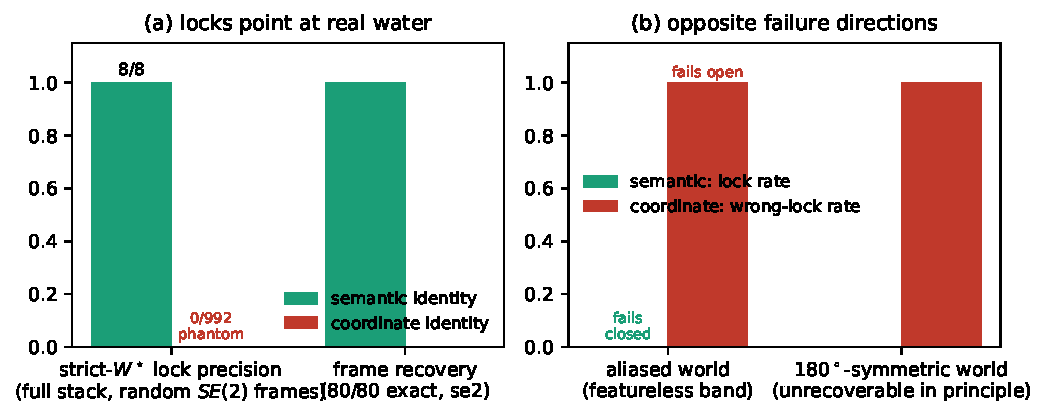
\includegraphics[width=0.92\linewidth]{figures/fig_route_identity}
\caption{Meaning-based identity under $SE(2)$ frames. \textbf{(a)}
Every strict-$\wstar$ lock the semantic stack makes points at real
water ($8/8$); the coordinate stack makes $992$ locks, all phantoms
($0/992$); frame recovery itself is exact in $80/80$
witness--traveler combinations. \textbf{(b)} The failure asymmetry in
worlds where identification is impossible (featureless band; a
$180^\circ$-symmetric layout where the frame is unrecoverable in
principle): semantic identity refuses to lock --- fails closed ---
while coordinate identity keeps confidently locking wrong cells ---
fails open.}
\label{fig:identity}
\end{figure}

\paragraph{The corner trap.} In the full stack, raw success is
non-discriminating under rotations (rotated coordinate poison mostly
maps off-grid and degrades into pseudo-exploration), so the
registered discriminator is \emph{warp-lock precision}: the share of
strict $\wstar$ locks pointing at real water. Before the void filter,
early border fingerprints (agents start in corners; rectangle borders
are $180^\circ$-symmetric) fed wrong-frame hypotheses and semantic
precision was $0.159$; with borders excluded as non-landmarks it is
\textbf{$1.000$ ($8/8$) vs.\ $0.000$ ($0/992$ phantom locks) for
coordinates}, with alignment onset in $100\%$ of episodes and clean
regressions on all earlier experiments
(Figure~\ref{fig:identity}).

\section{Related work}
\label{sec:related}

\paragraph{Map merging and place recognition.} Multi-robot SLAM
treats inter-map data association as an estimation problem over
metric features~\cite{cadena2016slam}; visual place
recognition~\cite{lowry2016vpr} matches appearance. Our contribution
is not a competing matcher but the measurement layer on top:
provenance-conditioned completion through recovered frames, the
fail-closed/fail-open asymmetry as a registered prediction, and law
invariance under frame removal.
\paragraph{Route sharing.} Stigmergy transfers paths anonymously
(pheromone gradients); learned communication (e.g.\
CommNet~\cite{sukhbaatar2016commnet}) transfers policies opaquely.
Neither exposes an edge-provenance decomposition, so neither can
state --- let alone predict --- where a transferred route breaks.
The rupture predictor is Time Warp~\cite{jefferson1985} thinking
applied to memory decay: deterministic replay of a gate over
calibrated kinematics.
\paragraph{Songlines.} The narrative frame is now load-bearing in
both directions: the song is a sequence (route warp), its places are
recognised by meaning (semantic identity), it fades verse by verse
(rupture law), and it protects the walker while it lasts (hazard
stratification). % TODO: add refs: ProcTHOR/ALFWorld for future substrates.

\section{Limitations and honest negatives}
\label{sec:limits}

(1) Grid worlds; translation and $90^\circ$ rotations only ---
continuous $SE(2)$ and appearance noise are future work (the
fingerprint threshold is exact-equality because the substrate is
noise-free; noisy substrates need the margin machinery of place
recognition). (2) Four registered predictions failed and are reported
with mechanisms: the $D{=}1$ negative control in ticks (turn economy;
exact in path length), gain monotonicity in $D$ (censoring; the truth
is a cliff), the full-stack success comparison under rotations
(non-discriminating; replaced by lock precision), and
``translation-fails-closed'' ($2/60$ fail open via symmetric
substructures). (3) The route follower is a new planner tier; all
three arms share it, but route-warp value is measured relative to
this consumer. (4) Hazard safety transfers by construction when the
witness's route is safe; the measured content is that place transfer
CANNOT carry it and that the protection ends at the predicted
rupture. (5) Scarcity-level completion of warp locks remains governed
by the collision phenomenology of the companion paper.

\section{Conclusion}

Strip the song down to a pin on a shared map and two things break
invisibly: the HOW (fatal at the first wall, expensive in every
hazard field) and the WHO-MEANS-WHAT (fatal under any frame
disagreement, and dangerous precisely because it fails open). Restore
the song --- edges with provenance, places with meaning --- and both
failures become measurable, lawful, and largely repaired: routes
transfer completion and safety and break only where the aging law
says; meaning recovers frames exactly, refuses honestly when the
world is ambiguous, and carries the entire measurement stack ---
$\varphi$, gates, distance law --- unchanged into a world where
agents share no coordinates at all. The pin was never the memory.
The song is.

\appendix

\section{Registered predictions and revisions}
\label{app:registered}
All predictions were written to disk before execution; the artifact
retains both versions wherever an operationalisation was revised.
Revisions: R1 negative control re-measured in path length; R1 gain
monotonicity re-formulated as cliff detection; W9 full-stack
discriminator changed from success to warp-lock precision; W8
strict-$\wstar$ functioning extended to include warp-assisted own
completions (taxi chains). % TODO: inline the registration JSONs.

\section{Reproducibility}
\label{app:repro}
\begin{verbatim}
PYTHONPATH=. python experiments/warp/exp_route_warp_r0.py
PYTHONPATH=. python experiments/warp/exp_route_warp_r1.py --seeds 20
PYTHONPATH=. python experiments/warp/exp_route_warp_r2.py --seeds 5
PYTHONPATH=. python experiments/warp/exp_route_warp_r3.py --seeds 20
PYTHONPATH=. python experiments/warp/exp_warp_semantic_identity.py
PYTHONPATH=. python experiments/warp/exp_warp_semantic_stack.py --seeds 20
PYTHONPATH=. python experiments/warp/exp_warp_rotation.py --seeds 10
\end{verbatim}

\begin{thebibliography}{9}

\bibitem[Cadena et~al.(2016)]{cadena2016slam}
C.~Cadena, L.~Carlone, H.~Carrillo, Y.~Latif, D.~Scaramuzza,
J.~Neira, I.~Reid, and J.~J. Leonard.
\newblock Past, present, and future of simultaneous localization and
mapping: Toward the robust-perception age.
\newblock \emph{IEEE Transactions on Robotics}, 32(6):1309--1332, 2016.

\bibitem[Jefferson(1985)]{jefferson1985}
D.~R. Jefferson.
\newblock Virtual time.
\newblock \emph{ACM Transactions on Programming Languages and Systems},
7(3):404--425, 1985.

\bibitem[Lowry et~al.(2016)]{lowry2016vpr}
S.~Lowry, N.~S\"underhauf, P.~Newman, J.~J. Leonard, D.~Cox,
P.~Corke, and M.~J. Milford.
\newblock Visual place recognition: A survey.
\newblock \emph{IEEE Transactions on Robotics}, 32(1):1--19, 2016.

\bibitem[Sukhbaatar et~al.(2016)]{sukhbaatar2016commnet}
S.~Sukhbaatar, A.~Szlam, and R.~Fergus.
\newblock Learning multiagent communication with backpropagation.
\newblock In \emph{NeurIPS}, 2016.

\end{thebibliography}

\end{document}
